\clearpage

\chapter{天琴对EMRI信号探测初探}

本章将介绍如何利用深度卷积神经网络算法构建天琴探测流水线,用以进行EMRI信号探测。主要内容分为四个部分。首先是数据的准备工作,包括信号建模,天琴仪器噪声建模,数据清洗等预处理工作;第二,进行数据的验证,验证模拟数据的正确性;第三,构建卷积神经网络模型,包括模型结构,目标函数及优化函数的选取等;最后,评估探测模型的性能和分析结果。




\section{准备数据}
%% 1. 介绍noisy signal 构造和noise only 样本的构造
%% 2. 正负样本的验证工作
%% 3、各个数据集的准备工作
在机器学习算法中,一般会准备3种数据集,分别是训练数据集、验证数据集和测试数据集。他们三个数据集完全不同,他们的作用也各不相同。训练数据集顾名思义用来训练神经网络算法,使得神经网络算法能够从中学习到数据的特性或特征。而验证数据集则用来检验神经网络学习效果,如果神经网络算法也能够正确辨别验证数据集,证明该算法正走向正确辨识数据类别的方向上。如果不能正确辨识验证数据集,则会用来惩罚该学习过程,使得学习过程能够修正方向。故而训练数据和验证数据一般是独立同分布(Independently Identically Distribution, IID )的数据构成。最后是测试数据集,这个一般是正式应用的数据集打包而成。而且最接近真实应用场景的数据,它一般只经过最少的数据预处理,用于检验前面训练得到的神经网络算法是否具备真实辨识能力和能做到什么样的程度。

在这个过程中,其实假设了真实数据的分布信息蕴含在数据中,但是有时候真实数据量很少,并不能完全分割为三种数据集,且我们并不知道数据真实分布信息。模拟的数据集假设服从更宽泛的分布范围,神经网络算法能从中学习,且能够应用于真实分布的测试数据。故而,我们采用的训练数据要尽可能采用更宽泛的分布模拟数据,用于检验该算法学习效果的验证数据集也采用跟训练数据一样的分布信息。测试数据集采用真实的观测数据或者最接近真实的模拟数据。具体来说,本文训练数据和验证数据中波形是采用同样随机分布得到所有引力波源参数(如中心黑洞质量都是采用log分布)产生的EMRI波形,而测试数据集则采用天文学模型得到引力波源参数来产生EMRI波形。之后都是以同样方式叠加模拟的高斯噪声,用来作为正样本。在三种数据集中正负样本各占一半,且负样本都是采用天琴噪声曲线的高斯噪声。



%按照前面关于卷积神经网络算法的介绍,这需要准备三种数据集,
概括来说,
一个是训练数据集,该数据集的大小一般没有上限,样本数量越充分,就越能更多表示EMRI信号的特点;一个是验证数据集,一般采用训练数据集大小的10\%,用于反馈训练效果;第三个数据集是测试数据集。三种数据集的准备过程基本完全一样,除了训练数据和验证数据会使用数据增强技术增加样本数量。
%以某个数据集的某个数据构建用以说明流程。
取训练数据的构建来描述数据的准备过程,数据准备工作基本流程如图\ref{fig:data_prep}
所示。
\begin{figure}[htbp]
 \centering
 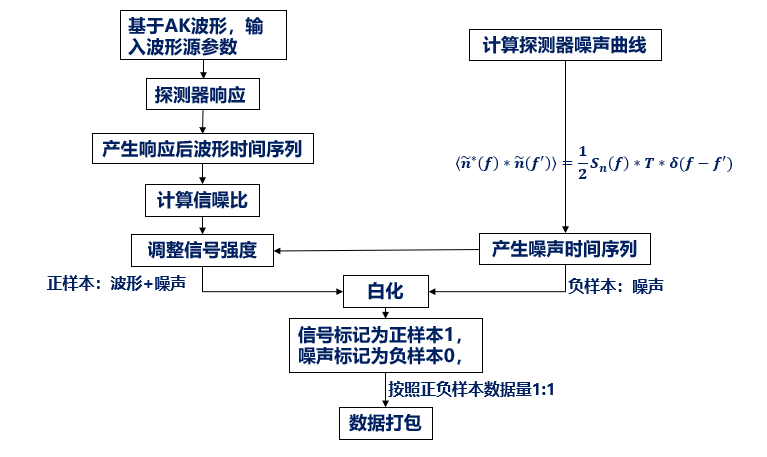
\includegraphics[width=1.1\linewidth]{data_prep}
    \caption{\label{fig:data_prep}训练数据准备流程图}
\end{figure}


%% targets: 由天琴噪声曲线产生高斯噪声

第一,介绍EMRI信号建模。采用AK波形来描述EMRI信号,需要设置14个物理源参数,如中心黑洞质量$\bf{M}$,小致密天体的质量$\bf{m}$等14个参数。在训练数据中,中心黑洞质量满足log分布($\sim log[10^4,10^7]M_\odot$),小致密天体的质量为10$\bf{M_\odot}$,其他的参数都服从均匀分布,具体源参数设置如表\ref{tab:AKW-sources}所示。
\begin{table}[htbp]
    \caption{\label{tab:AKW-sources}AK波形模型源参数取值范围}
    \wuhao
    \begin{tabularx}{\linewidth}{c|c|X<{\centering}}
        \hline
        参数符号 & 参数物理含义 &取值范围 \\ \hline
        M  & 中心黑洞质量 & log distribution[$10^4M_{\odot},10^7 M_{\odot}$]\\ \hline
        $\mu $ & 致密小天体  & 10$M_{\odot}$\\ \hline
        $a=S/M^2$ & 中心黑洞自旋 & uniform [0.5,1] \\ \hline
        $e_{lso}$ & 最内稳定轨道的偏心率值 & uniform [0,0.2]\\ \hline
        $\Phi_0$  & 初始相位 & uniform[$0.0,2*\pi$]\\ \hline
        $\alpha_0$  & 近日点进动角 & uniform[$0.0,2*\pi$]\\ \hline
        $\gamma_0$ & 轨道面进动角 & uniform[$0.0,2*\pi$]\\ \hline
        $\lambda$  & 轨道倾角 & cos($\lambda$)= uniform[-1,1]\\ \hline
        $\nu_{lso}$  & 最内稳定轨道截止频率 & 由$e_{lso}$决定\\ \hline
        $\theta_S$  & 黄道坐标下源的纬度 & uniform[$0.0,2.0*\pi$]\\ \hline
        $\phi_S$  & 黄道坐标下源的经度 & cos($\phi_S$)=uniform[$-1.0,1.0$]\\ \hline
        $\theta_K$  & 黄道坐标下中心黑洞自旋的纬度 & uniform[$0.0,2.0*\pi$]\\ \hline
        $\phi_K$  & 黄道坐标下中心黑洞自旋的经度 & cos($\phi_K$)=uniform[$-1.0,1.0$]\\ \hline
        $D_L$  & 初始光度距离 & $4.418*10^8$ [$\rm Psec$]\\ \hline
    \end{tabularx}
\end{table}

故而基于所有物理源参数的分布,可产生随机的源参数,采用AK波形得到模拟的EMRI源信号。之后基于探测器迈克尔逊低频近似响应,得到天琴响应后的EMRI信号。具体天琴响应方程式如公式所示。天琴响应主要影响极化角、方位角和多普勒平移的计算。

%说明极化角和多普勒平移的实际计算。
关于极化角$\psi_S$计算,$\bf{S}$表示源坐标下。具体公式计算如所示,实际带入天琴响应函数时,需要进行坐标转换,跟源方位角一样,都采用探测器坐标表示。
\begin{equation}
\tan \psi_S = \frac{\hat{L} \cdot \hat{z}-(\hat{L}\cdot \hat{z})(\hat{z}\cdot \hat{n})}{\hat{n}\cdot (\hat{L}\times \hat{z})}
\end{equation}
其中$\hat{L}$是轨道角动量方向的单位向量,$\hat{n}$是相对引力波波源传播反方向的单位向量。根据文献\cite{luo2016tianqin}, 天线响应函数中$\theta_S$不随时间变化,而$\phi_S$随时间变化。当$\phi_S$转换到探测器坐标系下,天琴的绕转周期为1天,即$\omega=2\times 10^{-5} rad/s$,则$\bar{\phi}(t)=\bar{\phi_0}+\omega t$。极化角$\psi_S$也会由于轨道角动量随时间变化而发生变化。
%多普勒平移
此外,因为探测器会随地球质心每年的周期运动而引入一个多普勒平移项,故而在时间域响应的信号上,相位多添加一项。则$\bar{\phi}_{\rm Doppler} (t)=\bar{\phi_0} +2\pi t/ T$,$\bar{\phi_0}$代表探测器在初始时刻$t=0$的位置,$T=1 year$表示地球绕太阳的轨道周期。

%说明EMRI波形产生速度慢,需要提前产生,计算一下产生效率的问题。
由于EMRI波形产生速度相对而言较慢,故而我们产生了$10^6$个模拟EMRI波形存储在硬盘。

%利用天琴噪声曲线产生模拟仪器噪声。
第二,产生模拟噪声。基于天琴探测器噪声曲线,产生高斯平稳的噪声序列。即利用噪声功率谱定义,产生模拟高斯噪声。
\begin{equation}
<\tilde{n}(f)\tilde{n}(f')>=\frac{1}{2}S_n(f)\times T_{obs} \times\delta(f-f')
\end{equation}
其中$\tilde{n}$表示频率域的噪声,$S_n(f)$是天琴噪声单边功率谱密度,具体表达式如公式表示,由文献\cite{luo2016tianqin}给出。$T_{obs}$表示观测时长。
\begin{equation}
S_n(f)=\frac{1}{L^2}\lbrack \frac{4S_a}{{(2\pi f)^4}} (\frac{1+10^{-4}Hz}{f}) + S_x \rbrack \lbrack 1+ 0.6((\frac{f}{f_*})^2)\rbrack
\end{equation}
$S_a$ 是加速度噪声, $S_a^{1/2}=1\times 10^{-15}m s^{-2}/\sqrt{Hz}$, $S_x$ 是位置噪声且 $S_x^{1/2}=1\times10^{-12}m/\sqrt{Hz}$, $f_*$ 是噪声极限且 $f_* =\frac{c}{2\pi L}$,$L$是探测器轨道臂长且$L=1.0\times 10^5 km$,$c$是光的传播速度。

产生频率域的噪声之后,由逆傅里叶变换可得到时间域的噪声序列。纯粹的噪声可以充当负样本,被标记为``0"。在时间域上,正样本由EMRI波形叠加噪声得到。并且正负样本都会经过白化操作并进行归一化。具体的白化操作表示如公式所示。
\begin{equation}
s = \frac{s}{\sqrt{S_n(f)}}
\end{equation}
其中$s$表示就是数据,如果是纯噪声,则$s(t)=n(t)$;如果数据含有信号,则$s(t)=h(t)+n(t)$,$h(t)$为时间域的EMRI信号模板。

%调整信噪比
第三,调整一个某信号的信噪比。由于EMRI信号非常复杂,显然其信号强度越弱,信噪比就可能越低,探测就越困难。为了简化EMRI信号探测问题,我们选取信噪比满足[50,120]的均匀分布的EMRI信号来构造数据集的样本。这里面涉及调整信噪比的操作。

当给定一个初始光度距离$D_L$和其他随机的物理源参数,能够产生一个初始响应后的EMRI信号,利用理想信噪比公式计算得到初始信噪比$\rho$。从均匀分布[50,120]中产生一个随机数$\rho_a$,由于波源距离与引力波强度成反比的关系,我们可以通过调整距离使得该波形强度调整为满足某信噪比的波形强度,即该波形新距离调整为$D_{\rm new}=\frac{\rho \times D_L}{\rho_a}$。理想信噪比的计算公式如\ref{exp:optimal_snr}所示,由于天琴可视作两个迈克尔逊干涉仪,则两个探测器对某一个引力波信号的总信噪比等于两个单独的信噪比的平方和后开方。
\begin{equation}\label{exp:optimal_snr}
\rho^2 = 4 \sum \frac{h(f)^2}{S_n(f)} df
\end{equation}

以上就是构建数据集中正负样本的基本过程,训练数据和验证数据是完全一样的准备过程,只是采用不同的源参数分布种子产生随机数,得到不同波形。但考虑由此得到数据集总数还不充分,还会通过数据增强技术增加样本数量。而测试数据集则没有用数据增强技术,但会采用其他源参数分布和波形模型用以构造不同的正样本,对最终的信号探测模型进行评估。


%数据增强
在训练数据和验证数据的准备上,尽管我们采用多进程产生波形,并且利用天河超级计算机的计算资源,产生EMRI波形的数量需求仍有所欠缺,而且考虑到存储的顾虑,因而我们也采用了数据增强技术,增加了训练数据和验证数据的正样本数量,用以增强探测模型的鲁棒性和避免卷积神经网络模型训练过程中出现过拟合问题。
具体的做法是,产生一个EMRI波形,训练过程中会产生 $n$个 噪声时间序列,且叠加到同一个EMRI波形上,则可以构造$n$个正样本(
$1\times n$),又免去存储的顾虑。
在本文实验中,采用$n=8$。实际上,数据增强技术在其他领域也发挥了举足轻重的作用,可详细参考文献[data-aug]

%其他源参数分布、波形模型
在测试数据集的准备上,会构造不同测试数据用以评估得到探测CNN模型的性能且不使用数据增强技术。测试数据集正负样本各一半。
%第一种,基于AK波形,采用与训练数据相同的源参数分布和信噪比分布($SNR \sim U[50,120]$) 产生的EMRI波形。第二种,基于AK波形,采用与训练数据相同源参数分布,但更广范围的信噪比分布,产生EMRI波形。第三种,基于AK波形,采用源参数的天文学分布,产生EMRI波形。第四种,基于AAK波形,采用与训练数据相同源参数分布和信噪比分布,产生EMRI波形。
其中负样本都是采用天琴噪声曲线产生的高斯噪声,满足独立同分布;而正样本模拟信号会由于模拟波形不同而不同,其样本概率分布会有所差异。模拟波形的不同影响因素有两种。一是波形模型,AK模型和AAK模型。二是波源物理参数,模拟联合概率分布(simulated joint probability)和源天文学分布(astronomical model)。其中还需要特别考虑模拟信号的强度不能太弱(信噪比),一方面在天文学模型中利用共动体积撒点得到光度距离,假如得到波源信噪比小于50,则丢弃;另一方面模拟源参数分布中可利用理想信噪比的计算来调整波源光度距离,从而选择合理的模拟波形。在这其中信噪比分布有均匀分布[50,120],也有从[10,130]取固定某个信噪比。

与训练数据相比较,基于以上两种影响模拟波形的因素可以构造6种测试模拟信号,具体模拟信号的情况如表\ref{tab:test-wave}。与此同时,也会产生跟模拟信号相同数目的模拟噪声样本。
\begin{table}[!htbp] 
\caption{测试数据集情况}  
\wuhao
\begin{tabularx}{\textwidth}
	{p{0.05\textwidth}%
	p{0.07\textwidth}%
	p{0.5\textwidth}%
	p{0.1\textwidth}%
	p{0.15\textwidth}}  % 10cm 減去前兩個欄位寬度後,剩下的通通給  
\hline                      % 第三欄位使用,文字超出的部份會自動折行  
类型 & 波形模型  & 源参数分布   & 模拟信号数目 & 评估指标  \\  
\hline  
1  & AK & 模拟联合概率分布, 信噪比服从均匀分布[50,120] & 500  & 混淆矩阵, ROC曲线  \\ 
2  & AK & 天文学模型 M12,信噪比大于50 & 500  & ROC曲线 \\ 
3  & AAK & 模拟联合概率分布, 信噪比服从均匀分布[50,120] & 500  & ROC曲线  \\ 
4  & AK & 模拟联合概率分布,固定信噪比[10,130] & 1000  & 有效性曲线\\ 
4  & AK & 固定MBH质量 $[10^4, 10^7M_{\odot}]$ & 1000  & 有效性曲线\\
5  & AK & 固定MBH自旋 $[0.0, 0.98]$ & 1000  & 有效性曲线\\
6  & AK & $\rm MBH\ 10^6M_{\odot},\rm spin\ 0.8$,固定红移 $[0.1,0.35]$ & 1000  & 有效性曲线\\
\hline  
\end{tabularx} 
\label{tab:test-wave} 
\end{table}  



\section{数据验证}
% 时间域高斯噪声满足高斯分布,且得到的时频图满足卡方分布。
在上一节的工作中,数据的准备工作就已经完成,但是数据质量决定了真实探测模型的起步和关键,所以数据验证工作就尤为重要。EMRI信号的验证通过计算信噪比和频率域图像来进行。噪声验证通过不同形式数据满足不同的分布特性来进行。

%展示一个数据样本:A和E画在同一个子图上
目前数据的正负样本如图和图所示。在时间域上,正样本由中心黑洞$10^6 M_{\odot}$-小天体$10 M_{\odot}$的双星系统得到EMRI信号构造而成。而负样本是纯噪声时间序列。白化前,负样本满足高斯分布(0,sigma),白化后,负样本满足N(0,1)的高斯分布。
\begin{figure}[!htbp]
 \centering
 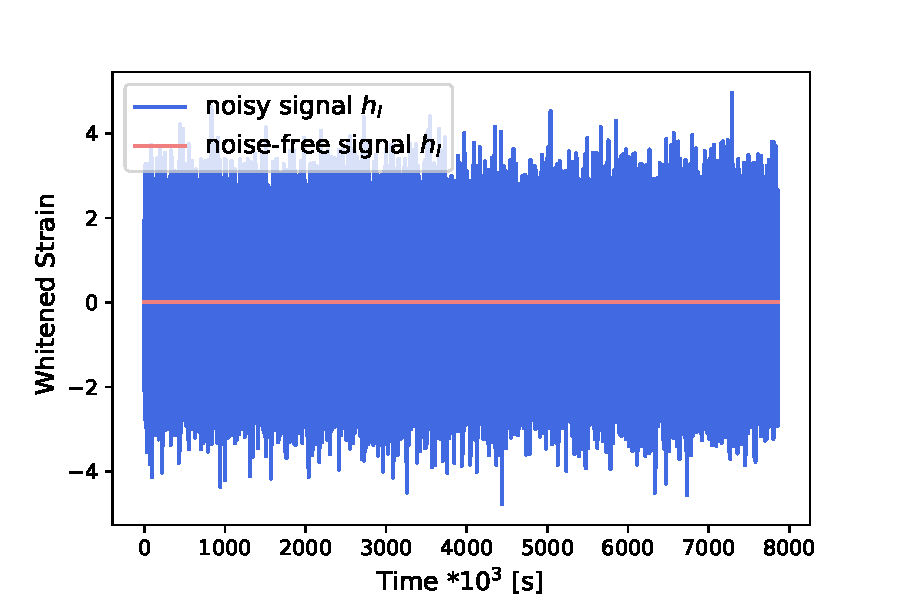
\includegraphics[width=.6\linewidth]{input-data-20210315.pdf}
    \caption{\label{fig:input-data}白化后的模拟信号样本和没有叠加噪声的模拟信号白化后的样本。天琴能够响应得到两个正交模拟信号,将其都经过白化操作,打包成一个正样本,数据维度为$(2 \times 262144)$}
\end{figure}



%高斯分布
以某一个时间域的噪声时间序列为例,白化前后都满足高斯分布,但两个高斯分布的标准差是不一样。
%开方分布
将时间域上的噪声用时频图进行转换,其功率值满足卡方分布,如图所示。自此验证了噪声模拟工作的正确性。

%在信号的模拟上,
在EMRI模拟信号的验证上,即验证波形的准确性。由于AK波形和AAK波形分别由文献\cite{chua2015improved}及其开源代码给出,主要添加探测器天线响应,我们通过取特定的方位角方式验证了响应函数的正确性,其中包括验证坐标系转换等工作。最后通过频率域图像,展示波形的正确性。将天琴的灵敏度曲线和某一个EMRI信号画在同一个图像上,并计算信噪比的合理性。


\section{构建卷积神经网络模型}
%描述模型结构
%训练策略

\subsection{模型结构}
在前人工作的借鉴下\cite{Hunter2018:PhysRevLett.120.141103, George:2016hay}, 设计了初始的神经网络结果,一步步进行训练测试得到了现在的卷积神经网模型。具体模型结构如图所示。一共有9层网络,3层卷积层,3层池化层,2层全连接层,1层输出层。

%模型结构
\begin{figure}[!htbp]
 \centering
 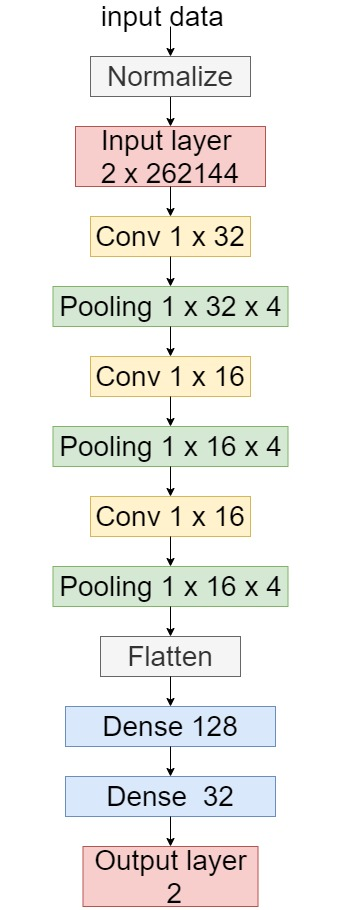
\includegraphics[width=.3\linewidth]{CNN-1}
    \caption[CNN模型结构]{\label{fig:CNN-arch}CNN模型结构。输入数据的维度是$(2 \times 262144)$,将输入数据输入CNN模型的输入层(Input layer)会采用两个通道读入该输入数据。经过三次的卷积(Conv)+池化(Pooling)作用,模型自动提取了特征。经过平铺(Flatten),把所有特征放到同一个维度上来表示。2层完成连接层(Dense layer)实现多层感知机的作用,将特征空间映射到2维的输出空间,从而得到该输入数据属于二分类中某个类别的概率。}
\end{figure}

具体实验环境中,搭建模型的实现和运行过程采用Python3.7、keras2.2.4 和 Tensorflow等软件,相对应的配置硬件环境是GPU Tesla V100 PCIe 16GB,
%CPU Intel Xeon Gold 6140 (72) @2.3,
%Memory 256GB, OS Ubuntu 18.04.4 LTS x86_64。


\subsection{训练过程}
实际训练过程中,模型过拟合问题不可避免[周志华,2016]\cite{zhou2016machine}\cite{ng2013unsupervised},但可以描述当前模型是否能够被接受。为了降低过拟合的影响,本文采用增加样本数据、添加dropout层的方法。具体为,在全连接层之前增加dropout层,参数设置为0.1。在训练数据中采用数据增强方法增加数据量,从而大大降低模型过拟合问题。在目标函数的选取上,选择了二分类交叉熵函数,其公式表示如式所示。
\begin{equation}
L=-\sum_{i=1}^{i=M}[y_i \log \hat{y_i}+(1-y_i)\log(1-\hat{y})]
\end{equation}
其中“L"表示目标函数损失值,``M"表示训练样本数目,$y_i$表示对应样本$i$的真实标签,$\hat{y_i}$对应样本$i$的预测标签。优化算法选择Ndam算法\cite{dozat2016incorporating}。

在训练过程中,由于单个数据大小约为4MB,考虑到内存(256G)和GPU存储容量(16G)的限制,选择了单批次训练数目为56个,设置训练300轮。这也意味着在每一轮训练中,每次会从全部训练数据中随机挑选56个数据进行训练,其中正负样本都各占一半。在具体训练过程中,也同时添加了提早结束训练机制(Early Stopping),假如验证准确率在50轮训练中没有任何提升,则结束模型训练。故而实际训练轮数会有所不同。

模型训练过程中的损失和准确率如图所示,图中展示训练150轮的训练和验证损失值,训练和验证准确率表现。当模型能够学习得到EMRI特征时,则无论是训练和验证损失值都会降低。但模型的实际表现会用测试数据集来评估。

最终训练数据为500000个,验证数据为50000个。

%\section{评估模型}
\section{分析结果}
%验证结果:信号处理分析指标、混淆矩阵、ROC曲线、AUC曲线
%基于本章第一节给出的四种测试数据,对训练得到的CNN模型进行了性能评估,描述的是受过训练以后的模型对未知数据的预测能力,也即泛化能力\cite{li2012s1, li2019s2}。经过训练后的CNN模型也可称为“分类器”或”判别器”。
经过训练后的CNN模型也可称为``分类器"(classifier) 或``判别器”,也称为``判别模型"。判别模型是由数据直接学习决策函数$Y=f(X)$或条件概率分布$P(Y|X)$作为预测模型\cite{li2012s1}。
%不能反映训练数据本身的特性,但它寻找不同类别之间的最优分类面,反映的是异类数据之间的差异。
%直接面对预测,往往学习的准确率更高。由于直接学习P(Y|X)或P(X),可以对数据进行不同维度上的定义特征、抽象化并使用,因此可以简化学习问题。


对训练得到的CNN模型进行了性能评估,描述的是受过训练以后的模型对未知数据的预测能力,也即泛化能力\cite{li2012s1}\cite{li2019s2}。而给出性能评估,就要构造合理评估模型性能的测试数据集,所有的结果都应该基于没有经过训练的测试数据进行检验。因此针对这个分类器的性能评估,实质上就是要分析该模型$Y=f(X)$[$P(Y|X)$]是否合理,从概率角度,我们应该让通过采用更接近真实数据概率分布得到测试样本对模型进行测试。即采用上一节内容中所说的六种测试数据对CNN模型进行测试,并采用相应的评估标准进行展示。


%总结评估指标
参考一般用于信号探测和机器学习算法的评价指标(measure)\cite{li2012s1},本文采用正确率(accuracy),查全率(Recall),查准率(Precision),ROC(Receiver Operating Characteristic)曲线,有效性曲线(efficiency curve)
来分析模型表现。
%误报率(false alarm probability), 漏报率(false missals probality),

对每一个测试数据集,都能得到其经过分类器后的类别结果,也即混淆矩阵(Confusion Metrix)。在这其中,``TP"(True Positive)表示正样本正确分类为正样本的数量,即信号正确分类为信号的数量;``TF"(True Negative)表示为负样本正确分类为负样本的数量,即噪声正确分类为噪声的数量,这两类的结果落在矩阵对角线,对角线的数量越多证明分类模型性能越好。同理可知“FP"(False Positive)表示噪声被错分为信号的数量,``FN"表示信号被错分到噪声的数量。

\begin{table}[!htbp]
\centering
\wuhao
\begin{tabular}{|c|c|c|}
%\begin{tabularx}{\linewidth}{c|X<{\centering}}
\hline
\diagbox{真实标签}{预测标签}&正样本&负样本\\ %添加斜线表头
\hline
正样本&TP&FN\\
\hline
负样本&FP&TN\\
\hline
\end{tabular}
\end{table}



\subsection{准确率、查全率、查准率}
准确率是数据被正确分类的概率,包含信号正确识别为信号,噪声正确识别噪声。具体表达式如公式所示\cite{li2012s1}。
\begin{equation}
\rm Accuracy = \frac{\rm TP+ \rm TN}{\rm TP+\rm FN+\rm FP+\rm TN}
\end{equation}
查准率是正样本被正确分类的数目占全部预测正样本数目的比例。
\begin{equation}
\rm Precision= \frac{\rm TP }{\rm TP+\rm FP}
\end{equation}
查全率,又被称做召回率,表示正样本被正确分类的数目占全部真正正样本数目的比例。
\begin{equation}
\rm Recall = \frac{\rm TP}{\rm TP+\rm FN}
\end{equation}

准确率是描述广泛问题的通用指标,但是由于不同应用场景下会有一些偏好,所以需要同时参考查准率和召回率。在引力波信号探测中,由于引力波信号比较微弱,所以我们更希望不要漏掉可能的引力波信号,故而召回率会更加被偏重考虑。综合考虑查准率和查全率有所侧重,可以引入一个新指标F-score。
\begin{equation}
\rm F-score = (1+\beta^2)   \frac{\rm Precision}{\rm Recall}{\beta^2(\rm Precision + \rm Recall)}
\end{equation}
其中$\beta$是权重系数。当$\beta=1$, 意味着查准率和查全率并重,则该F值是它们两者的调和平均值记为$F_1$,且表达式如下所示。
\begin{equation}
\rm F_1 = \frac{2\times \rm Precision\times \rm Recall}{(\rm Precision+ \rm Recall)}=\frac{2}{\frac{1}{\rm Precision}+\frac{1}{\rm Recall}}
\end{equation}


以跟训练数据独立同分布的1000个测试数据为例,其中500个信号,500个噪声,得到的混淆矩阵如图\ref{fig:cm-iid}所示。%将六种数据类型\ref{tab:test-wave},
得到的汇总准确率等结果指标如表\ref{tab:acc}所示。
\begin{figure}[!htbp]
 \centering
 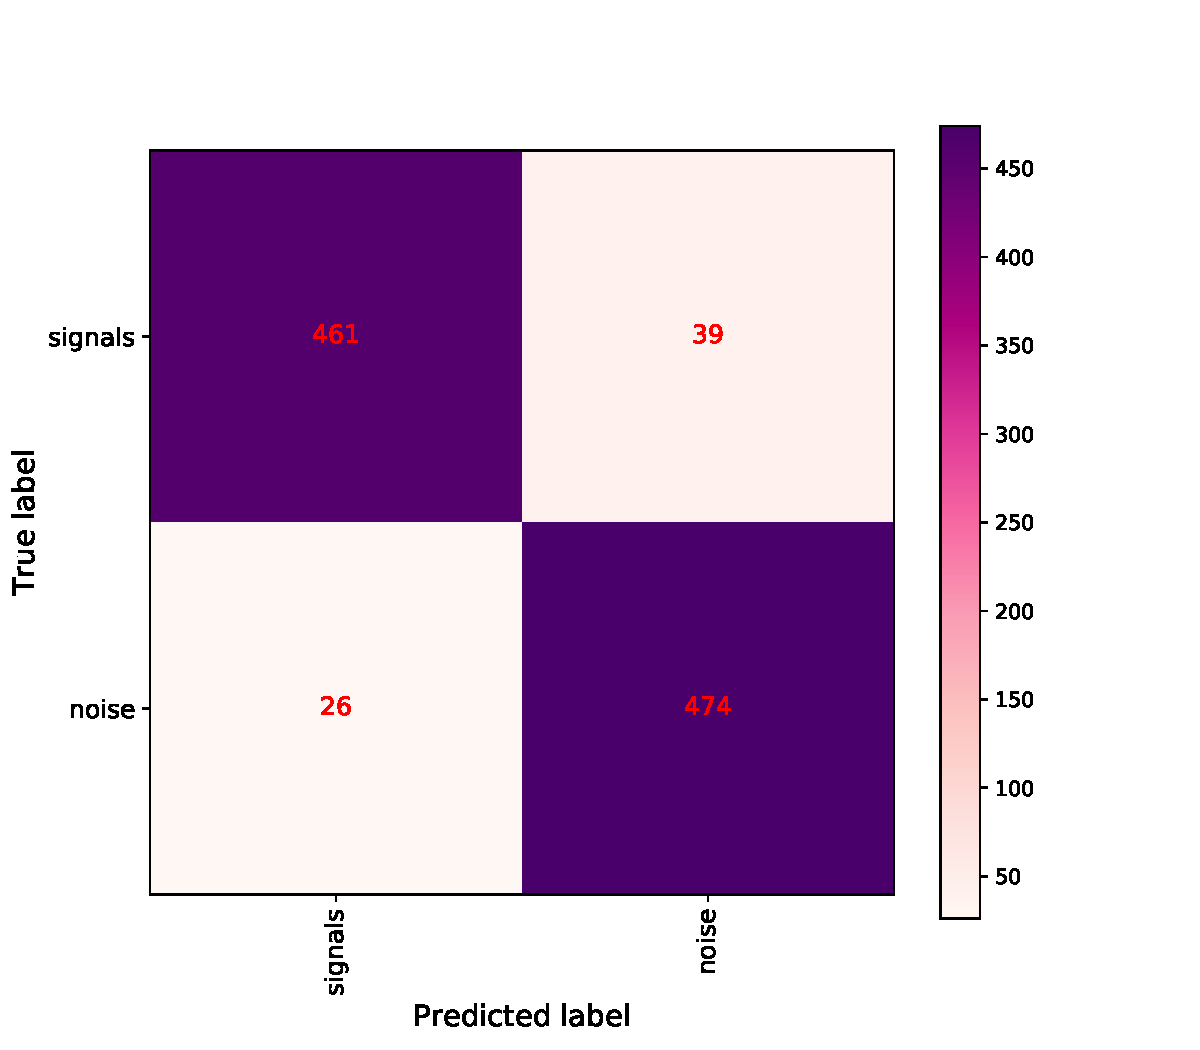
\includegraphics[width=.6\linewidth]{lisatools-AK_cm-20210315-2.pdf}%{lisatools-AK_cm.png}
    \caption{\label{fig:cm-iid}与训练数据独立同分布测试数据}
\end{figure}

\begin{table}[!htbp]
\centering
\wuhao
\begin{tabular}{|c|c|c|c|c|c|}
\hline
%\diagbox{数据集类型}{}&正样本&负样本\\ %添加斜线表头
测试数据集类型&数据数量&准确率&查准率&查全率&$F_1$\\
\hline
类型 1&1000&91\%& & &\\
\hline
\end{tabular}
\label{tab:acc}
\end{table}
%不同类型说明在[准备数据]该节内容有说明。

\subsection{ROC曲线}
ROC曲线表示随着误报率阈值的变化,真正率(True Positive Rate,TRP)和相对应假证率(False Positive Rate,FPR)的变化。针对某一个误报率阈值,如误报率(False alarm Rate)为0.1时,以假正率为横轴,真正率为纵轴,得到的曲线越往左上角,表明分类器得到误报率设置相对较低时,真实探测率相对较高,意味着分类器的性能越好。

基于AK波形,与训练数据独立同分布产生波形源参数得到EMRI信号的测试数据,分类器得到的ROC曲线如图\ref{fig:ROC-astro}和图\ref{fig:ROC-AAK-iid}中蓝线所示所示。两图中的蓝线是一致的。当固定误报率为1\%时,真值率约为90\%。

基于AK波形,与训练数据源参数分布不同,采用天文学分布产生波形源参数模拟得到EMRI信号的测试数据集,其中模拟信号不会调整其信噪比,分类器得到ROC曲线如图\ref{fig:ROC-astro}红线所示。从图中可以看出,相比于蓝线,误报率越低,红线的真值率也会更低。固定误报率为1\%时,红线的真值率为72\%左右。细致分析了该红线的测试数据集,发现其包含的模拟信号都是信噪比约为50的信号,故而真值率会比较低。

\begin{figure}[!htbp]
 \centering
 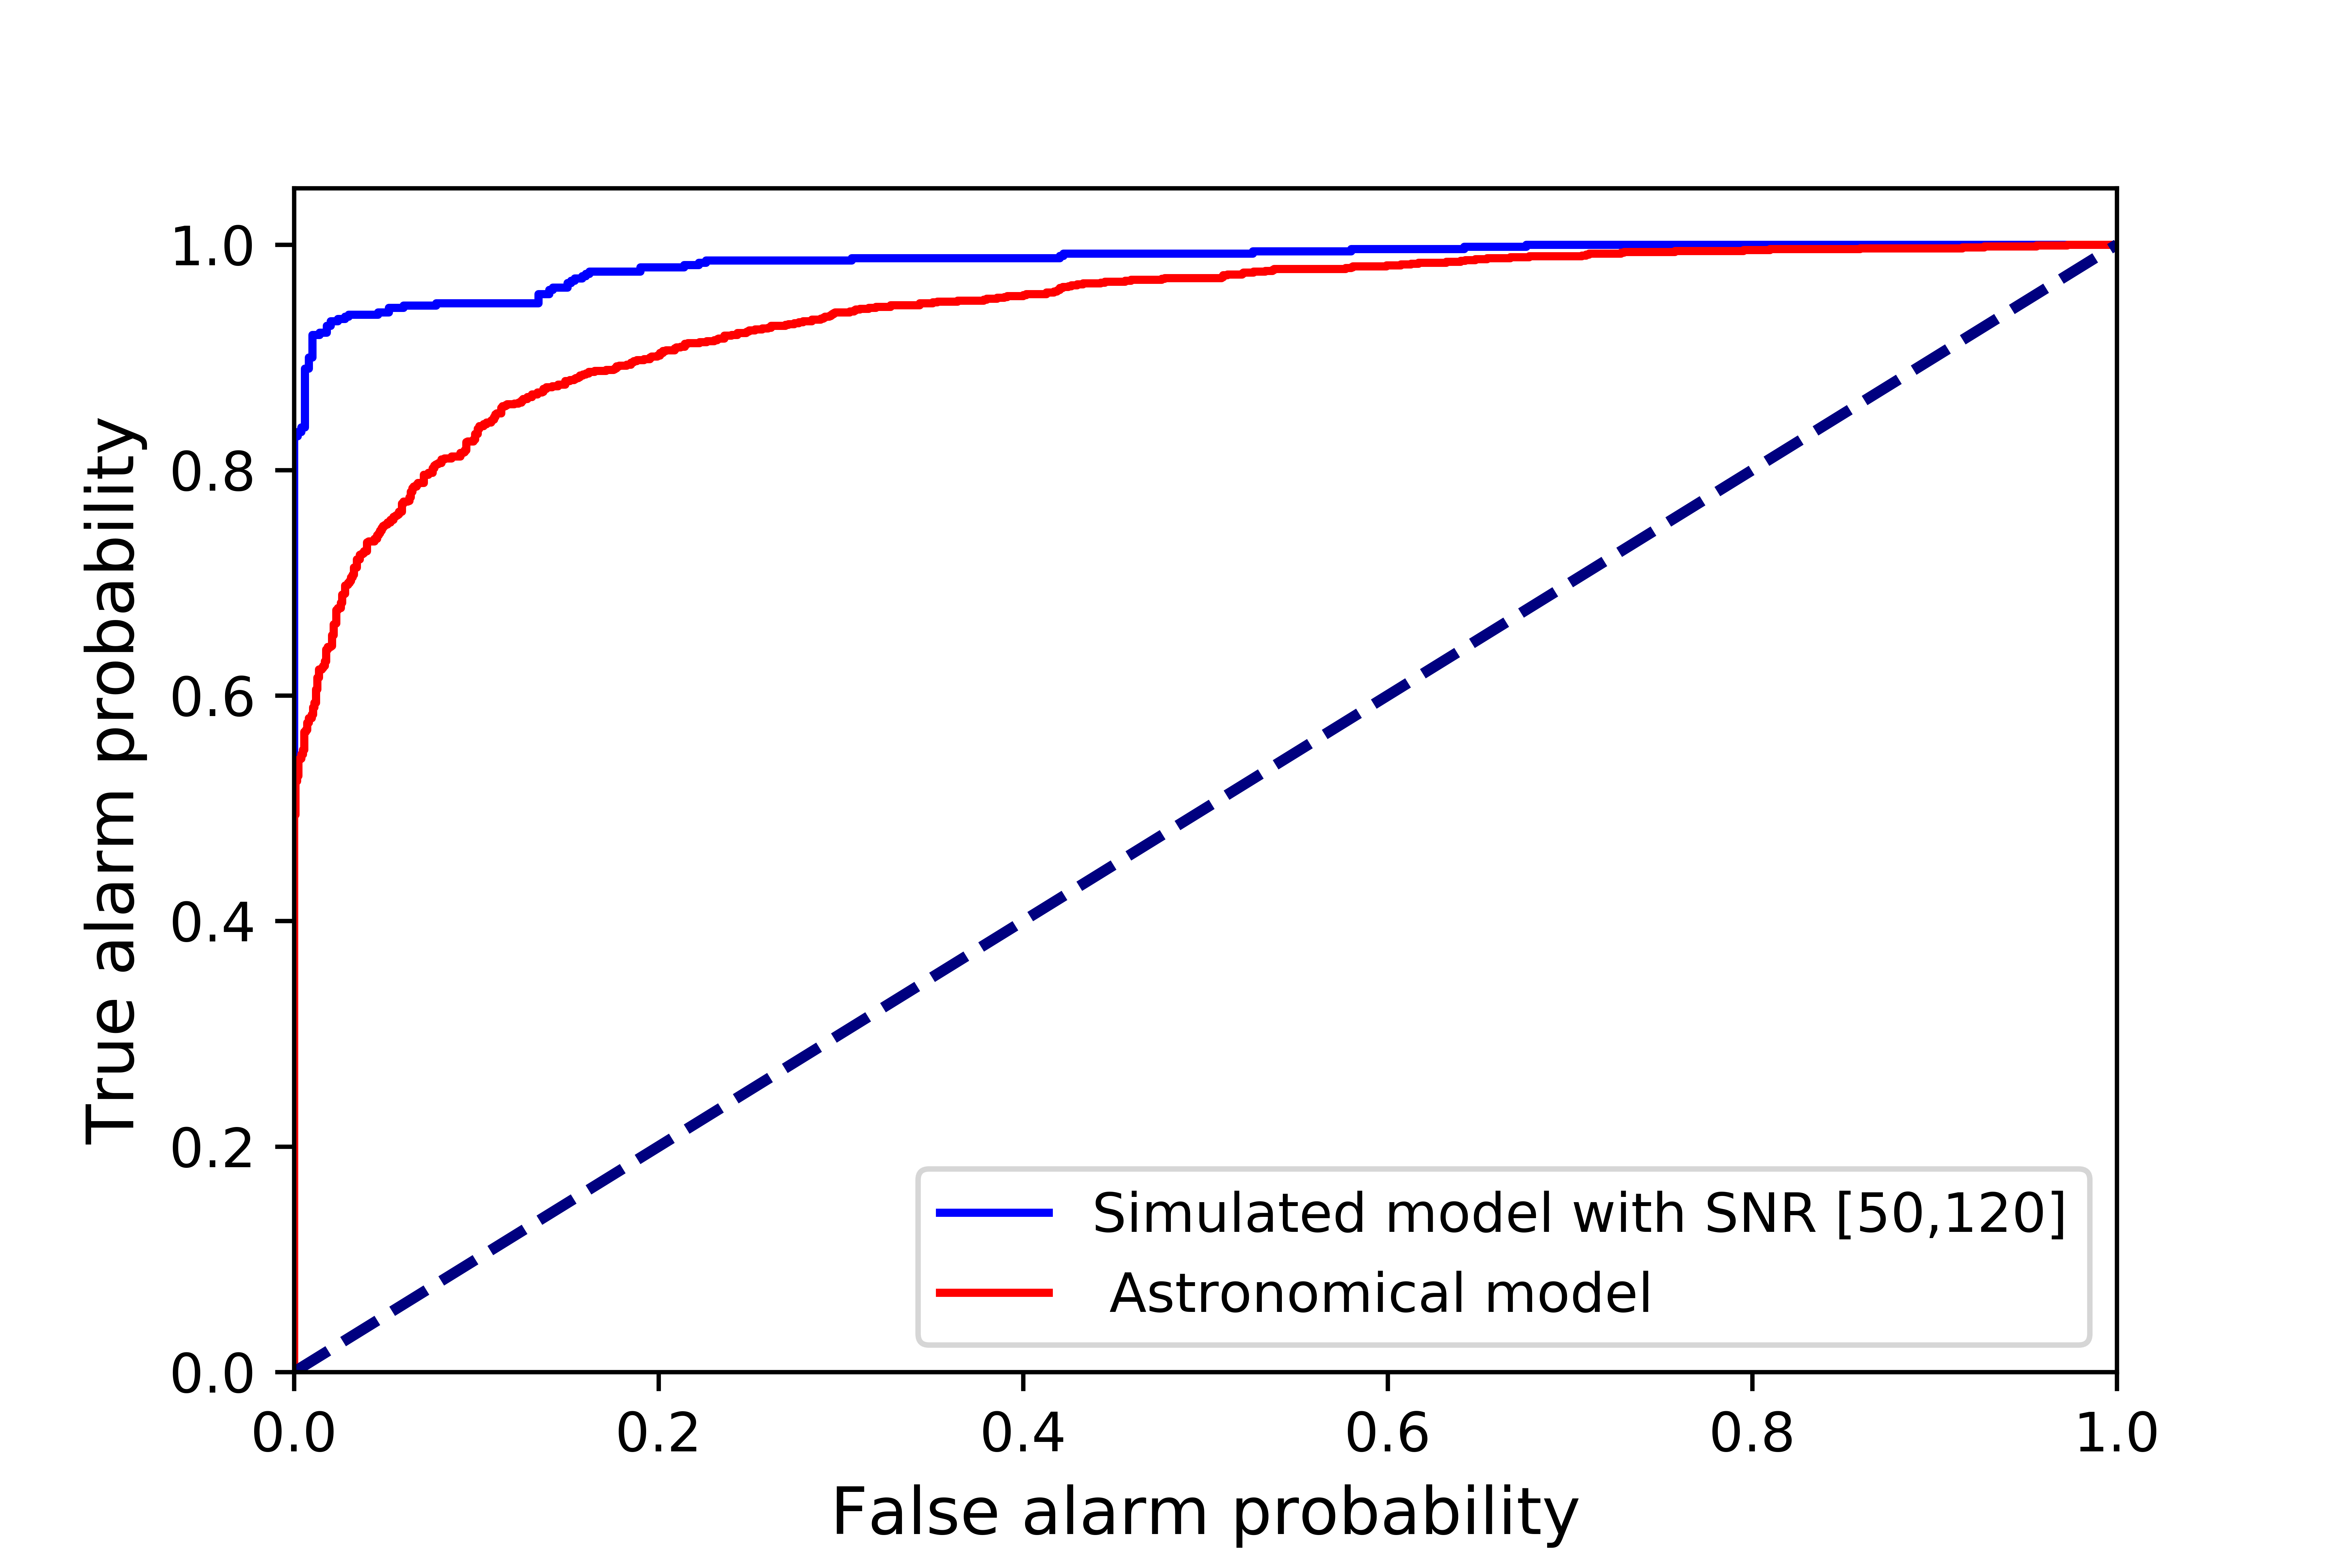
\includegraphics[width=.8\linewidth]{0113-M12-ROCcurve.png}
    \caption{\label{fig:ROC-astro}采用天文学模型模拟得到的EMRI信号测试得到的ROC曲线}
\end{figure}


基于AAK波形,与训练数据独立同分布产生波源参模拟得到EMRI信号的测试数据,即模拟信号的产生除了更换波形模型,源参数的选取跟训练过程中的模拟信号采用同样分布。则分类器得到的ROC曲线如图中\ref{fig:ROC-AAK-iid}红线所示。相比于蓝线,红线与蓝线取得基本一致的结果。这表明采用AK波形和AAK波形所模拟的EMRI信号他们具备了基本一致的EMRI信号特征,这跟原本波形模型的特点是一致的。AAK波形模型就是在参考时间上对相位进行了校准(时间维度的相位偏移),但是保持了AK波形对EMRI信号所建模的相位特点。故而他们能取得一致结果也是可以验证的。
\begin{figure}[!htbp]
 \centering
 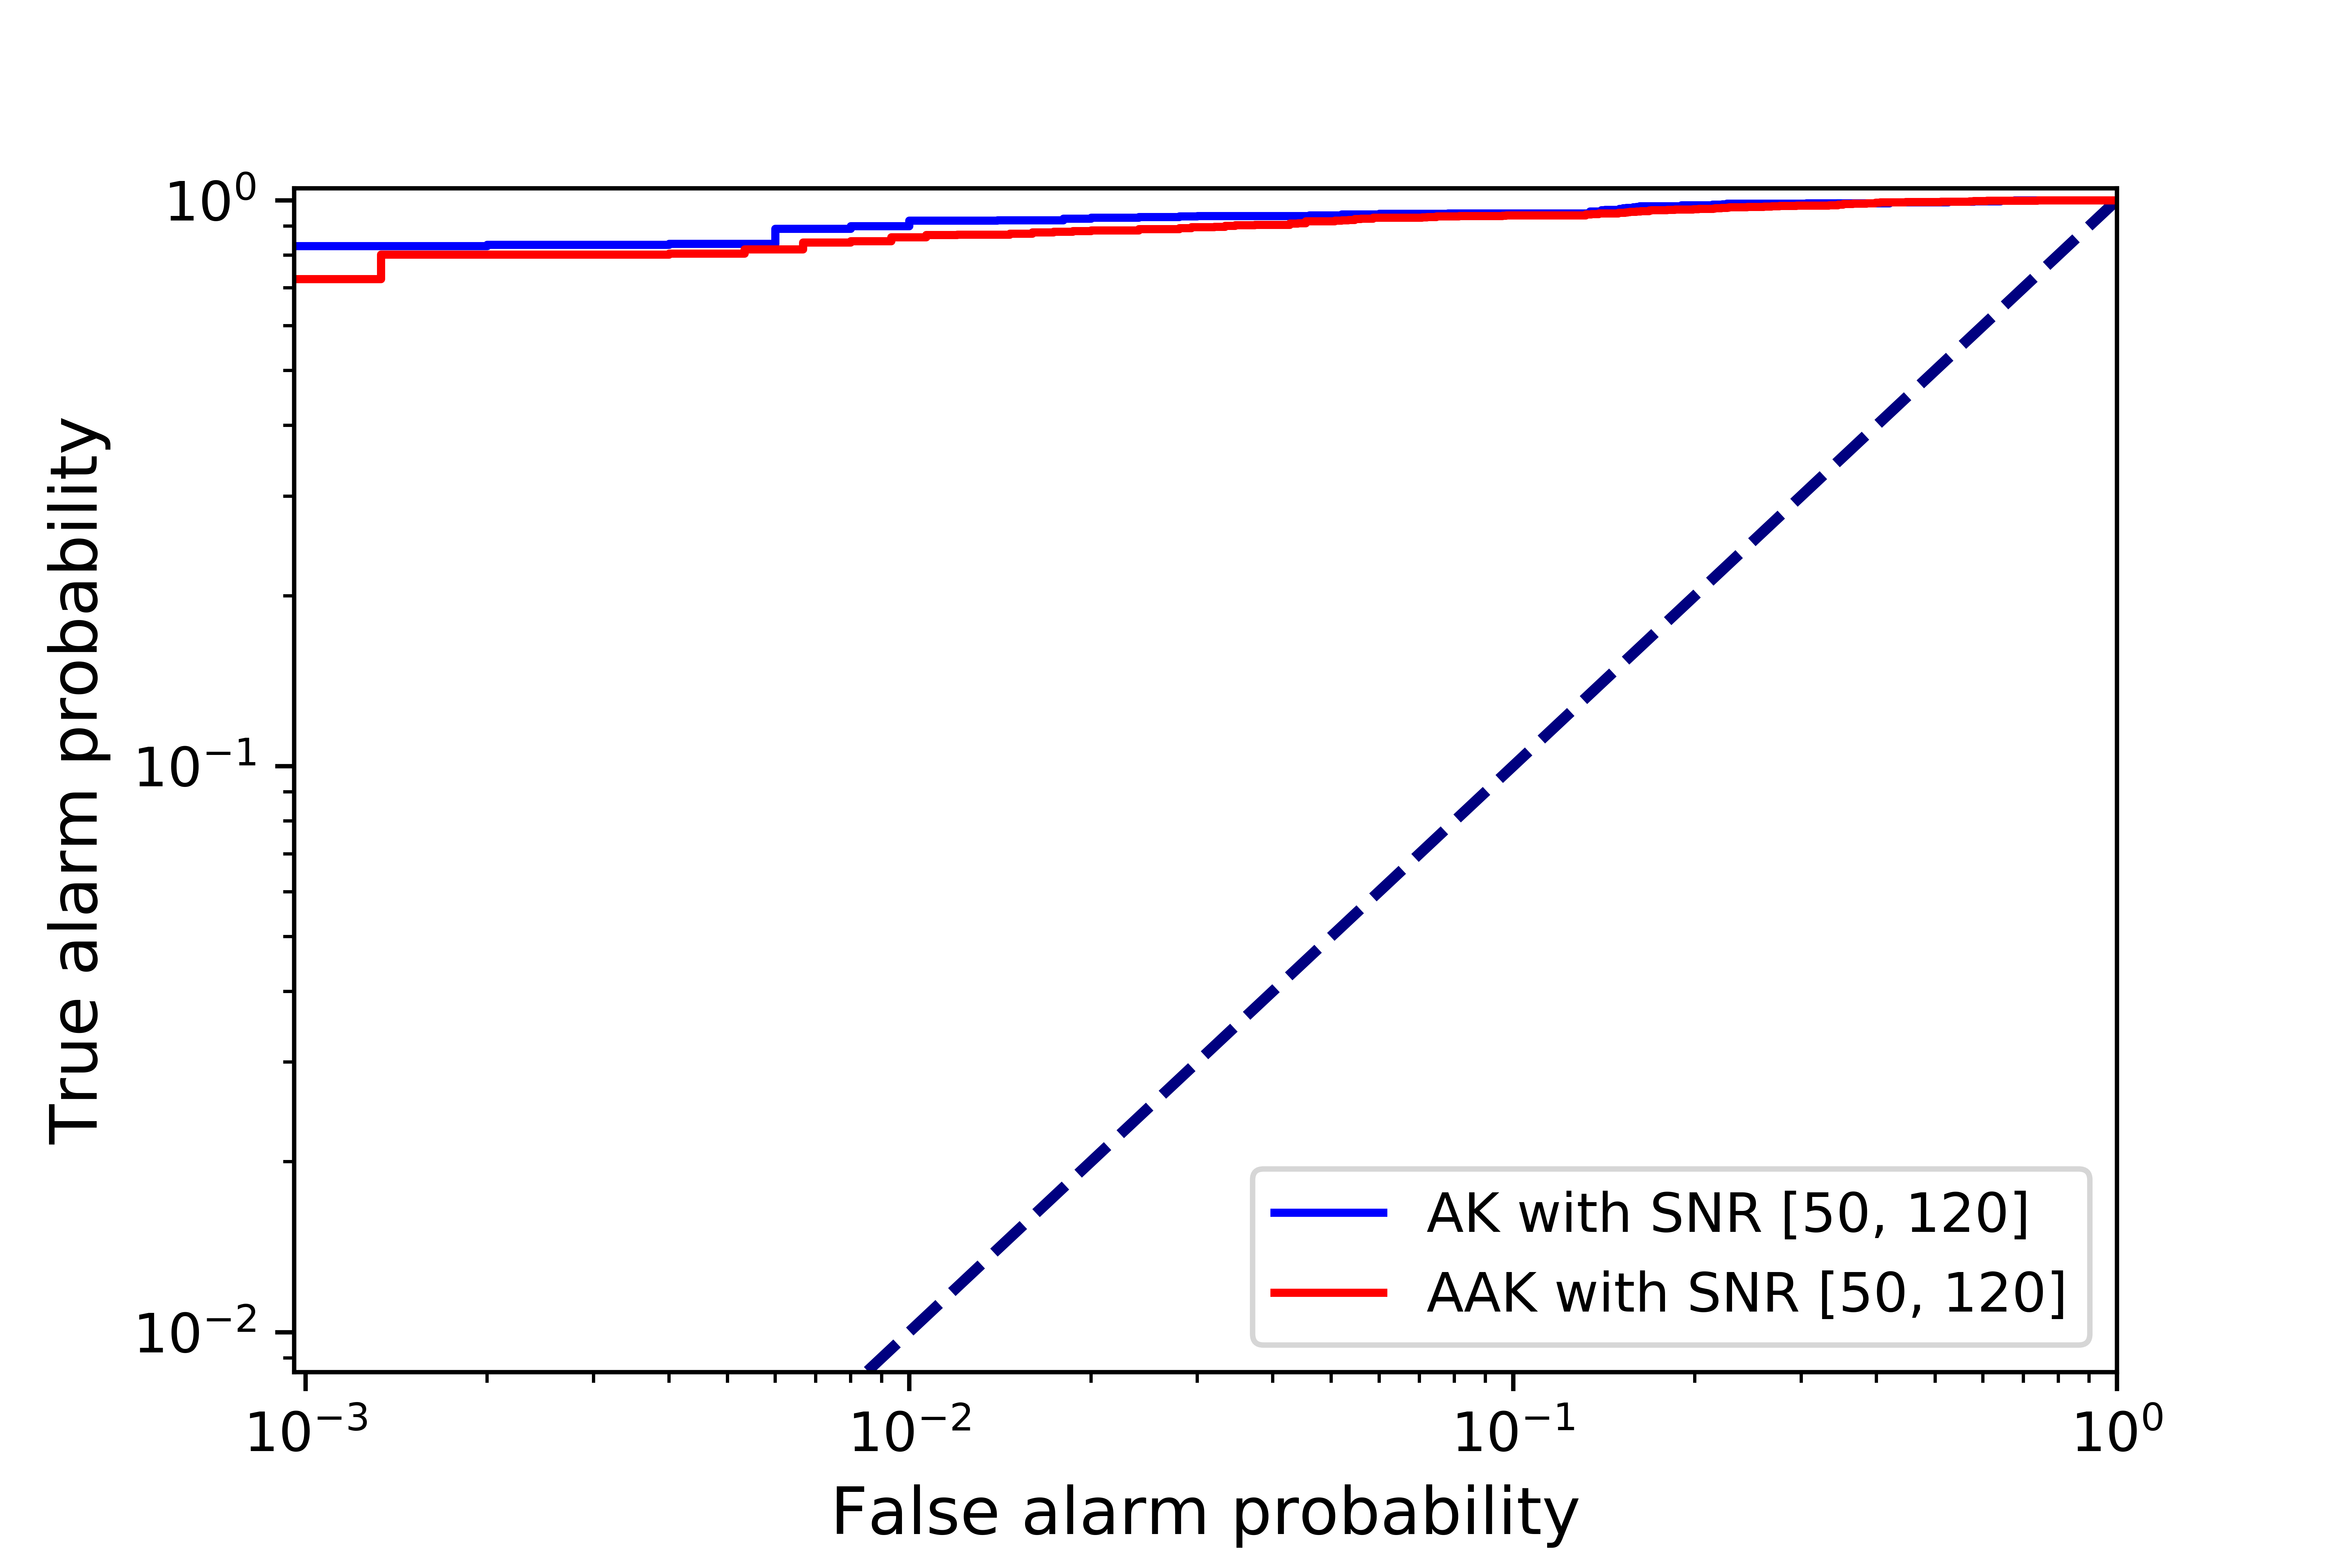
\includegraphics[width=.8\linewidth]{0113-ROC-AAK-AK.png}
\caption{\label{fig:ROC-AAK-iid}基于AAK波形模拟的EMRI信号测试得到的ROC曲线}
\end{figure}

\subsection{有效性曲线}
基于ROC曲线的定义,取固定误报率的前提下,基于AK 模拟的EMRI波形,用以查看对CNN模型对不同源参数的灵敏度变化。在本文中,构造了信号信噪比、中心质量黑洞质量、自旋参数不同的测试数据集,用以测试CNN 模型得到的真正率变化,即类型4-6的测试数据集\ref{tab:test-wave}。

第一,构造了固定信噪比不同的EMRI波形,比如构造了信噪比为10的EMRI信号和信噪比为130的EMRI信号,各2000个。把这两个数据集都用该分类器进行测试性能,分别设置误报率为1\%和0.1\%时,得到两个真正率(TPR)。同理可以构造其他固定信噪比的数据集,得到相应的真正率,绘制有效性曲线,结果如图\ref{fig:EC-SNR}所示。
\begin{figure}[!htbp]
\centering
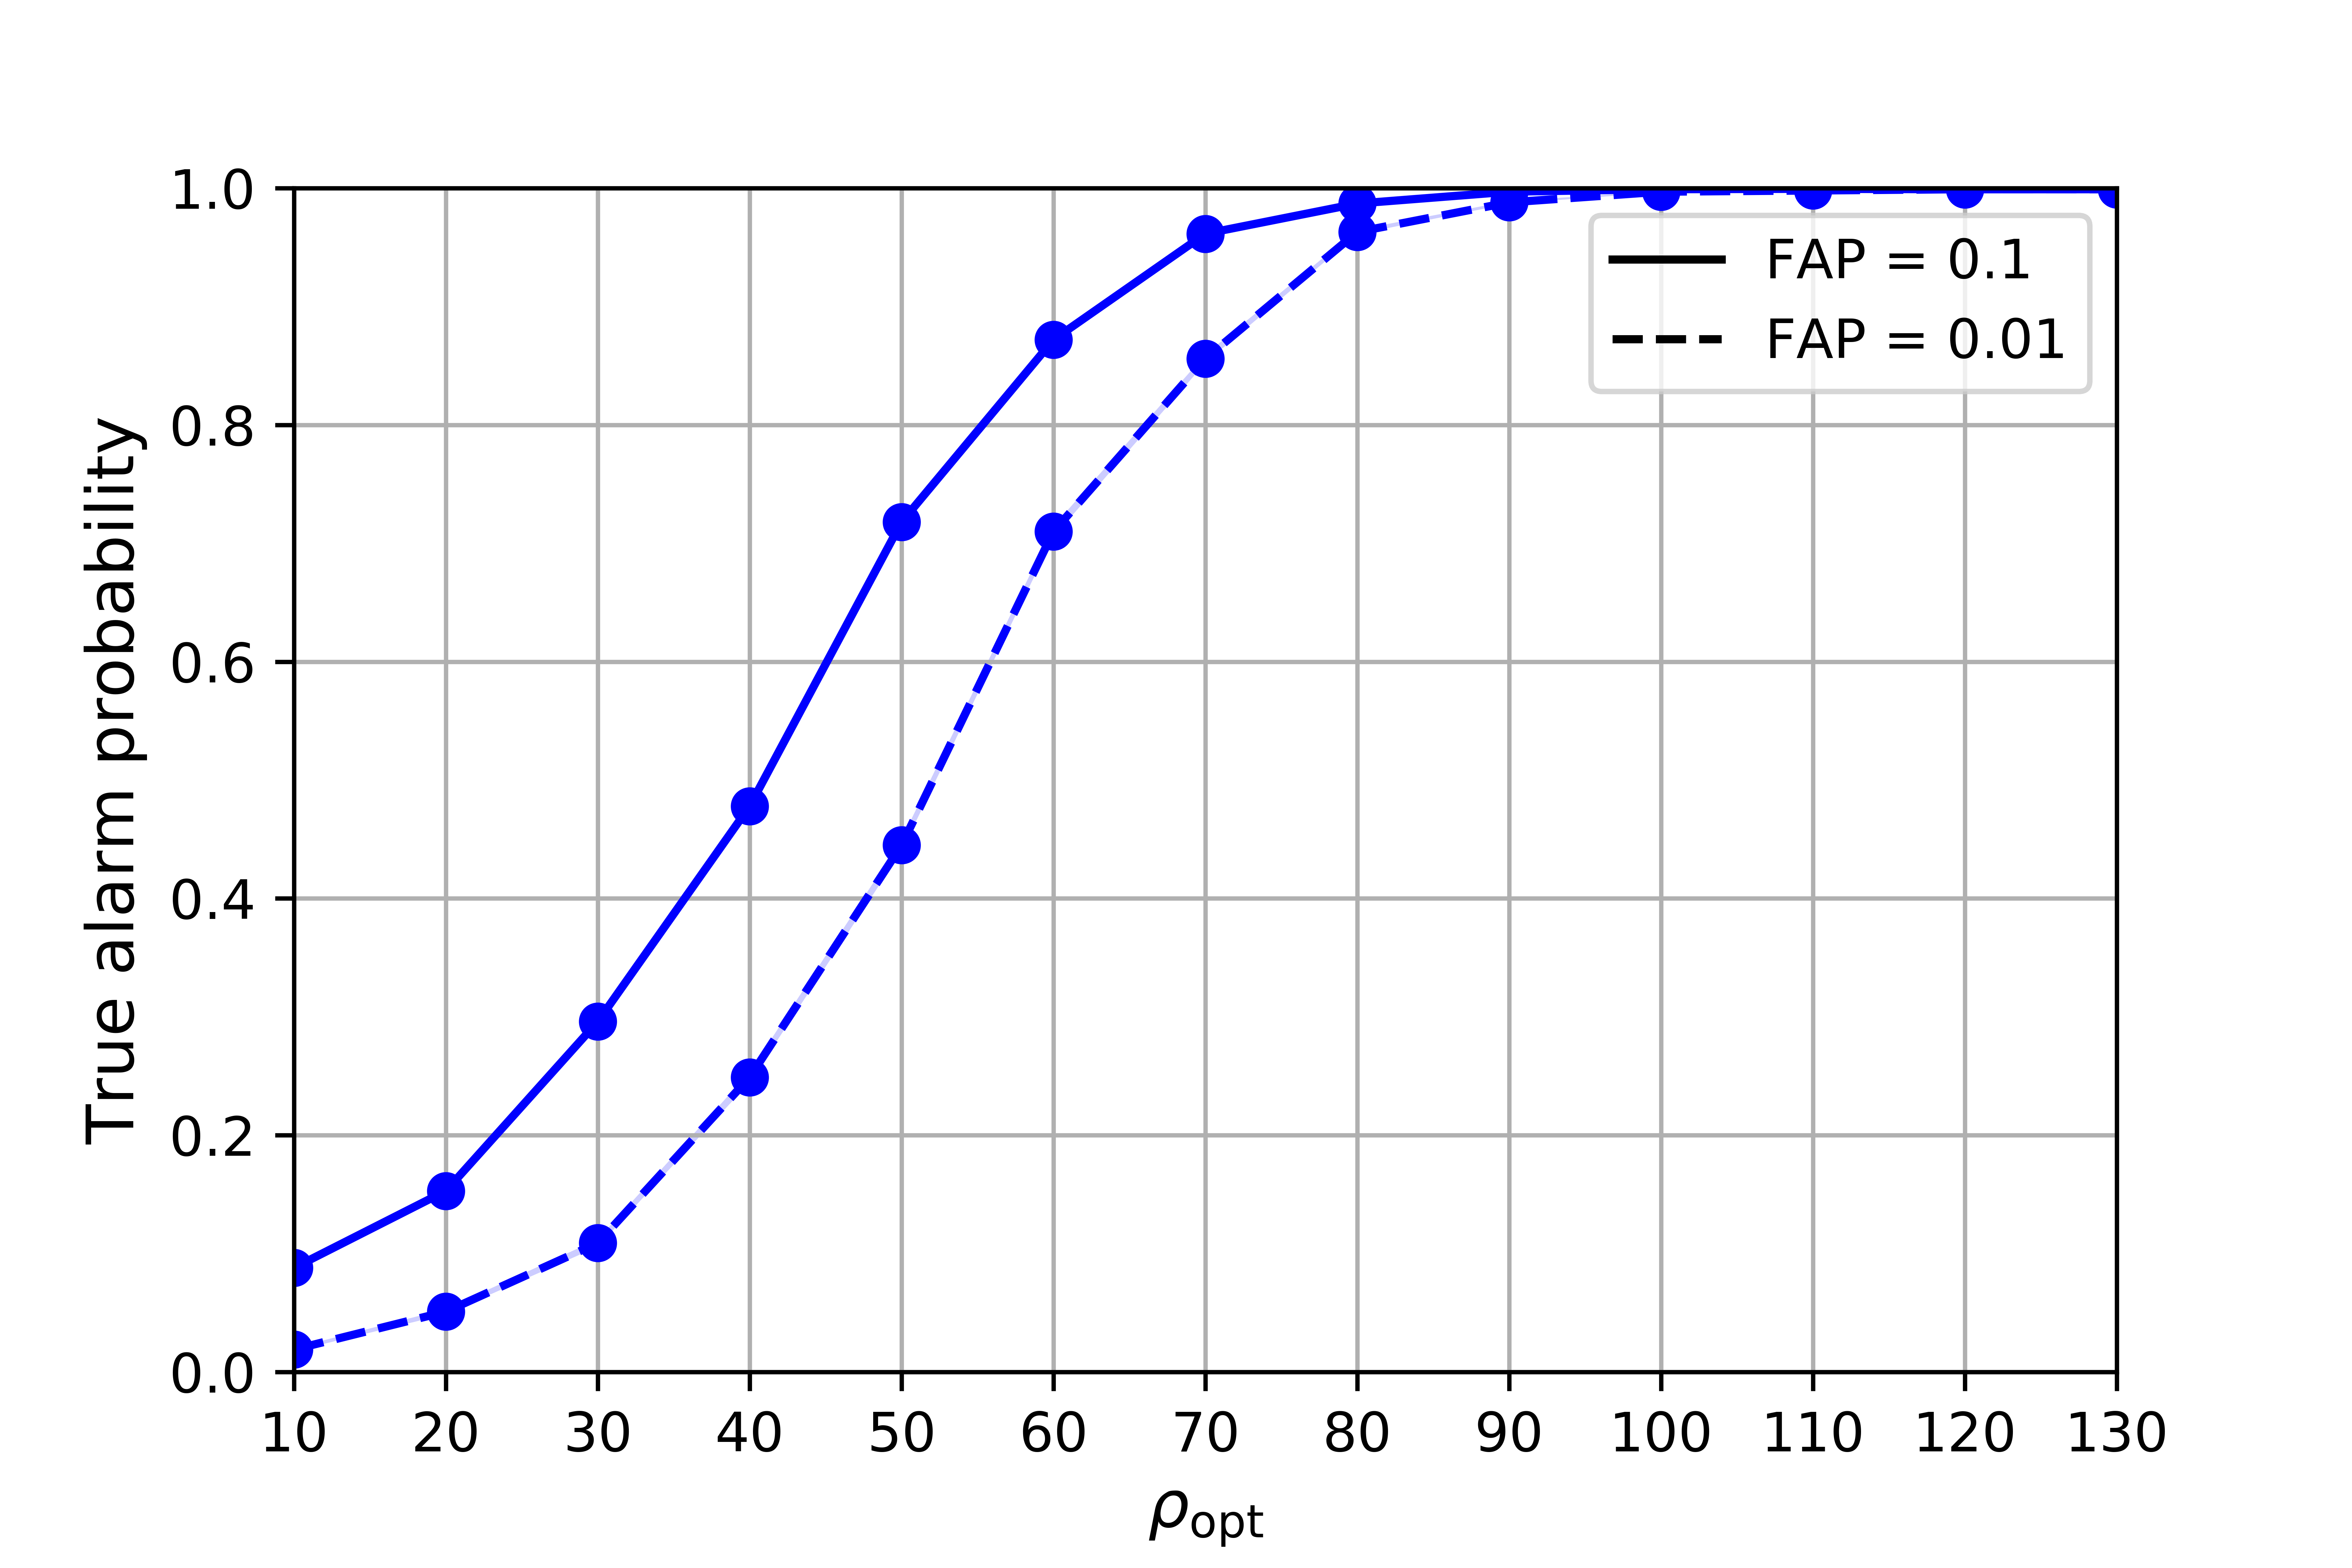
\includegraphics[width=.8\linewidth]{efficiency-SNR.png}
\caption{\label{fig:EC-SNR}有效性曲线:含有固定信噪比不同模拟信号的测试数据集}
\end{figure}

第二,构造了不同固定中心黑洞质量的EMRI波形的数据集。其中自旋固定为0.98,其他源参数随机产生。每个测试数据集数目为2000个,其中1000个模拟信号,1000 个模拟噪声。得到的真正率随中心黑洞质量该参数变化的曲线,结果如图\ref{fig:EC-SMBHmass}所示。
\begin{figure}[!htbp]
 \centering
 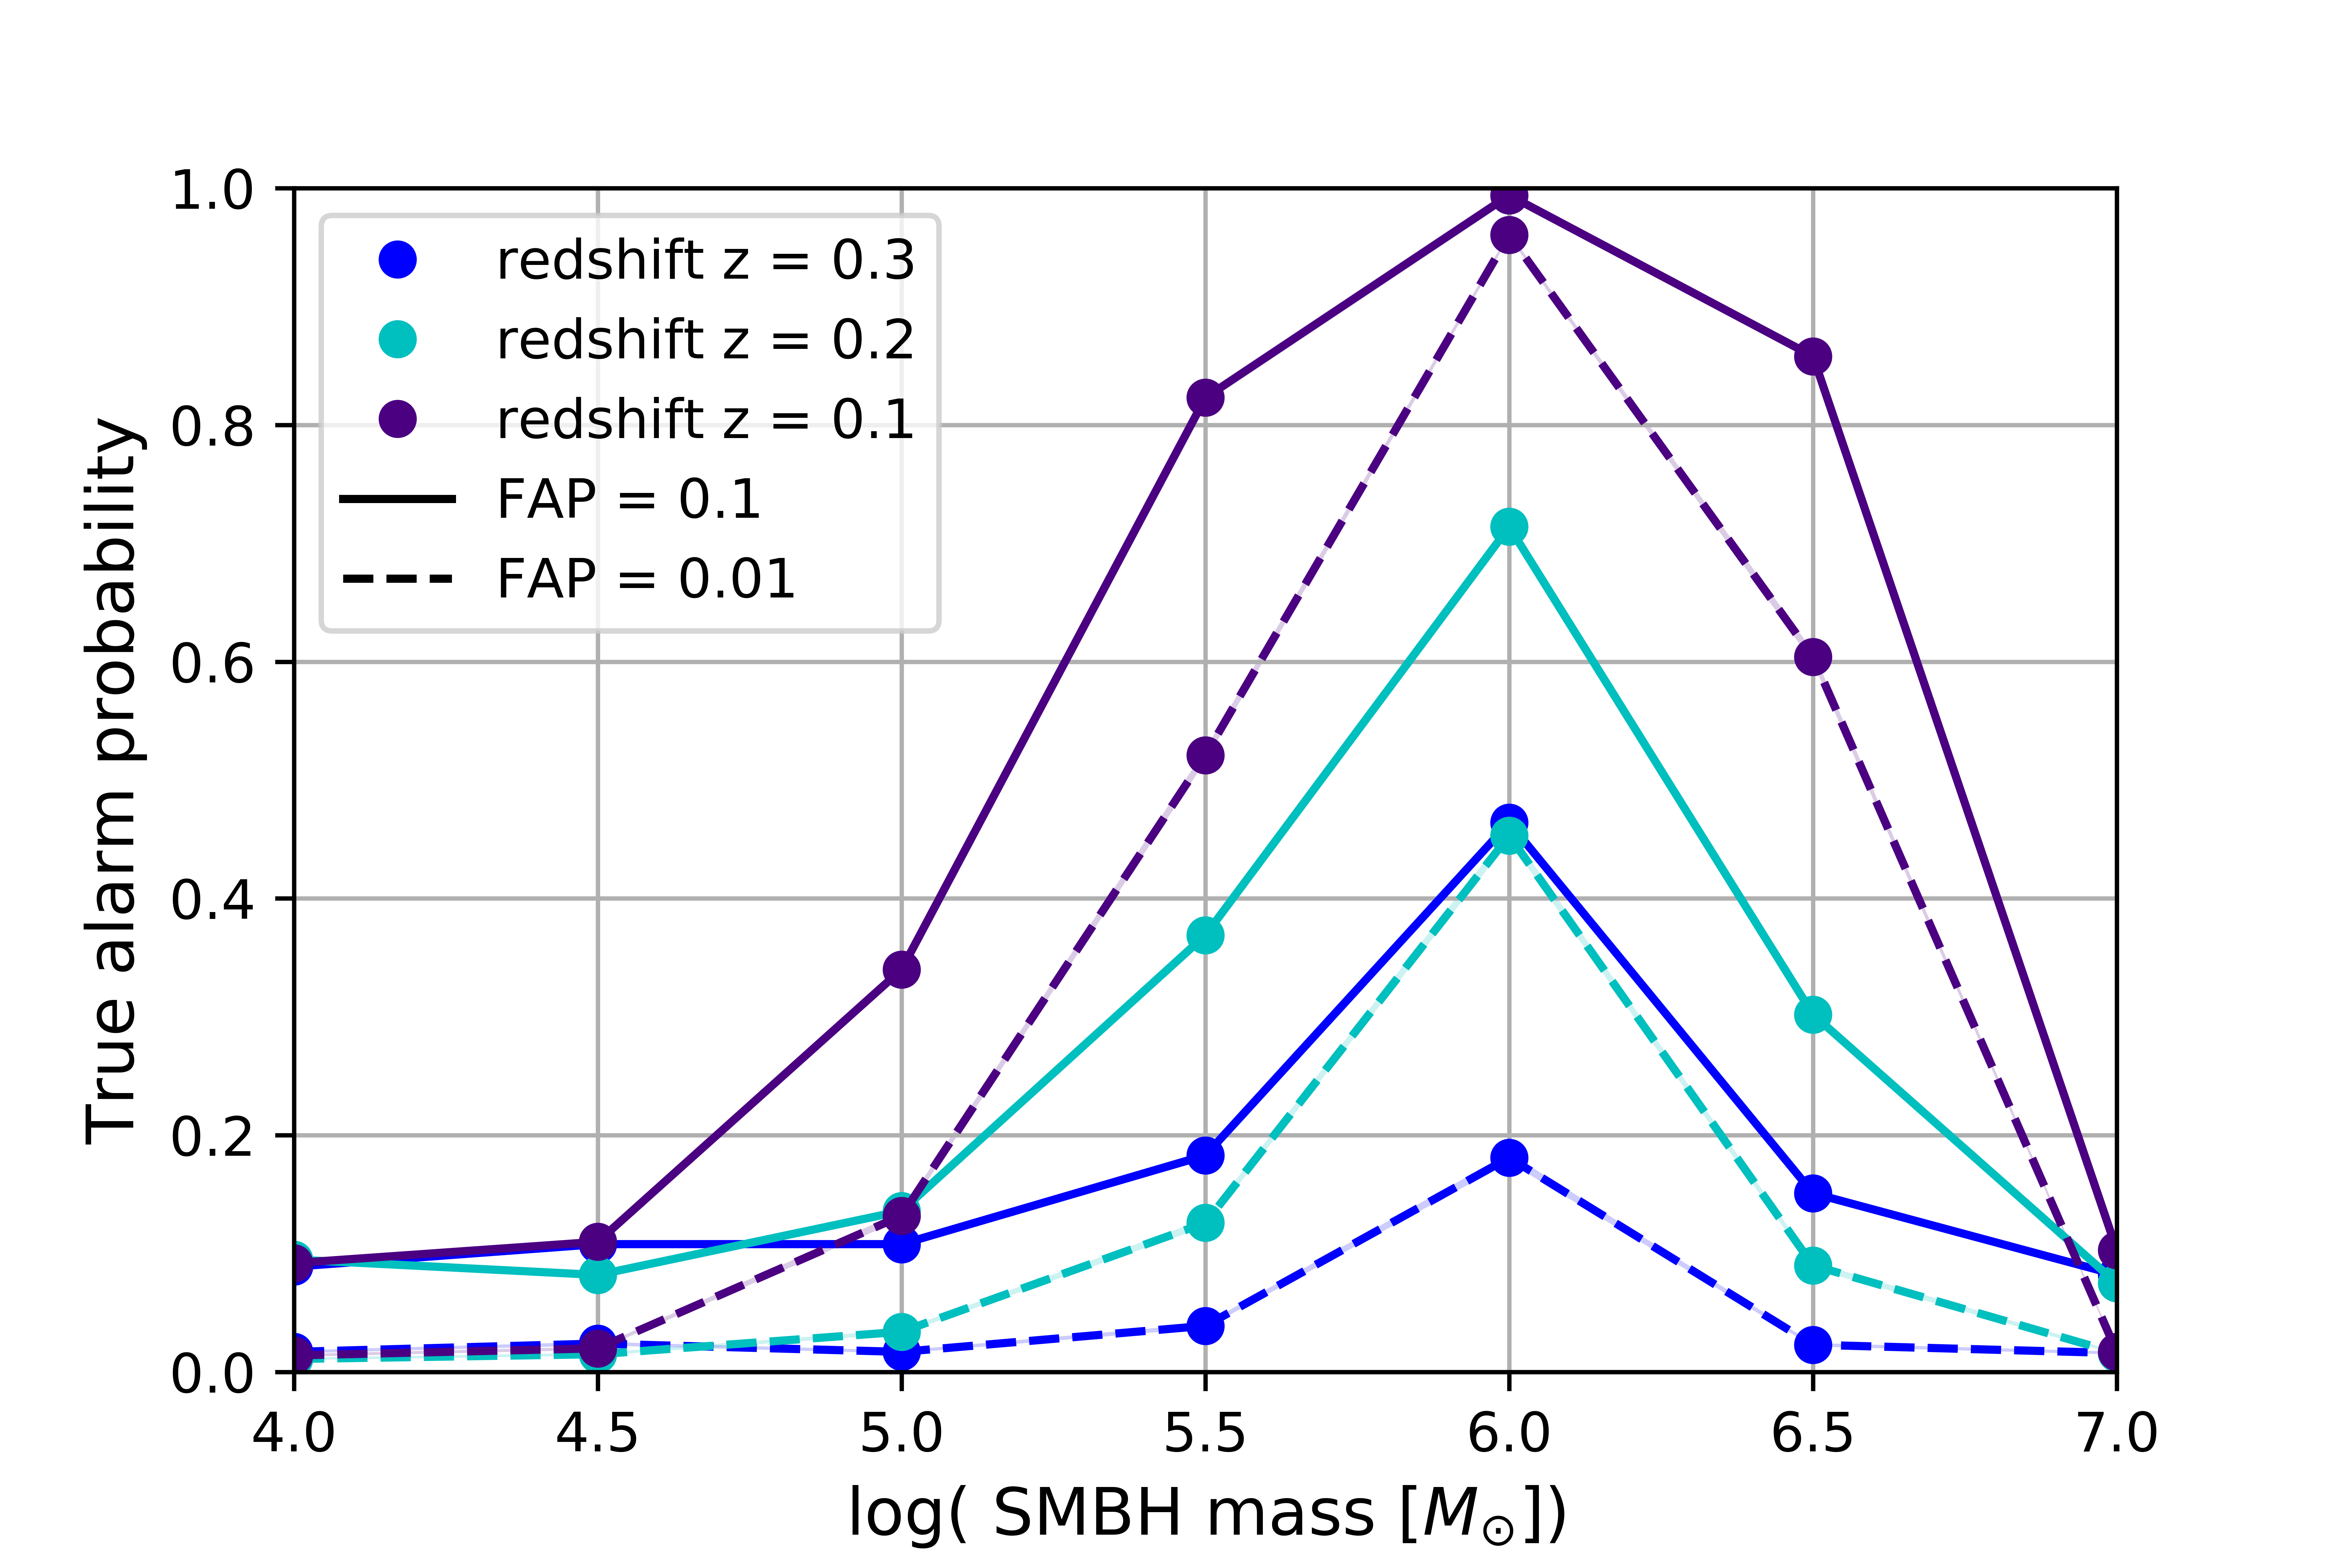
\includegraphics[width=.8\linewidth]{efficiency-SMBHmass.png}
    \caption{\label{fig:EC-SMBHmass}有效性曲线:含有固定中心大质量黑洞不同模拟信号的测试数据集}
\end{figure}

第三,构造了不同中心黑洞自旋的EMRI波形的数据集。设置中心大质量黑洞为$10^6 M_{\odot}$,其他源参数随机产生,不调整信噪比。同理,每个测试数据集数目也为2000个,模拟信号和模拟噪声各占一半。则得到的真正率随中心黑洞自旋该参数变化的曲线,结果如图\ref{fig:EC-Spin}所示。
\begin{figure}[!htbp]
 \centering
 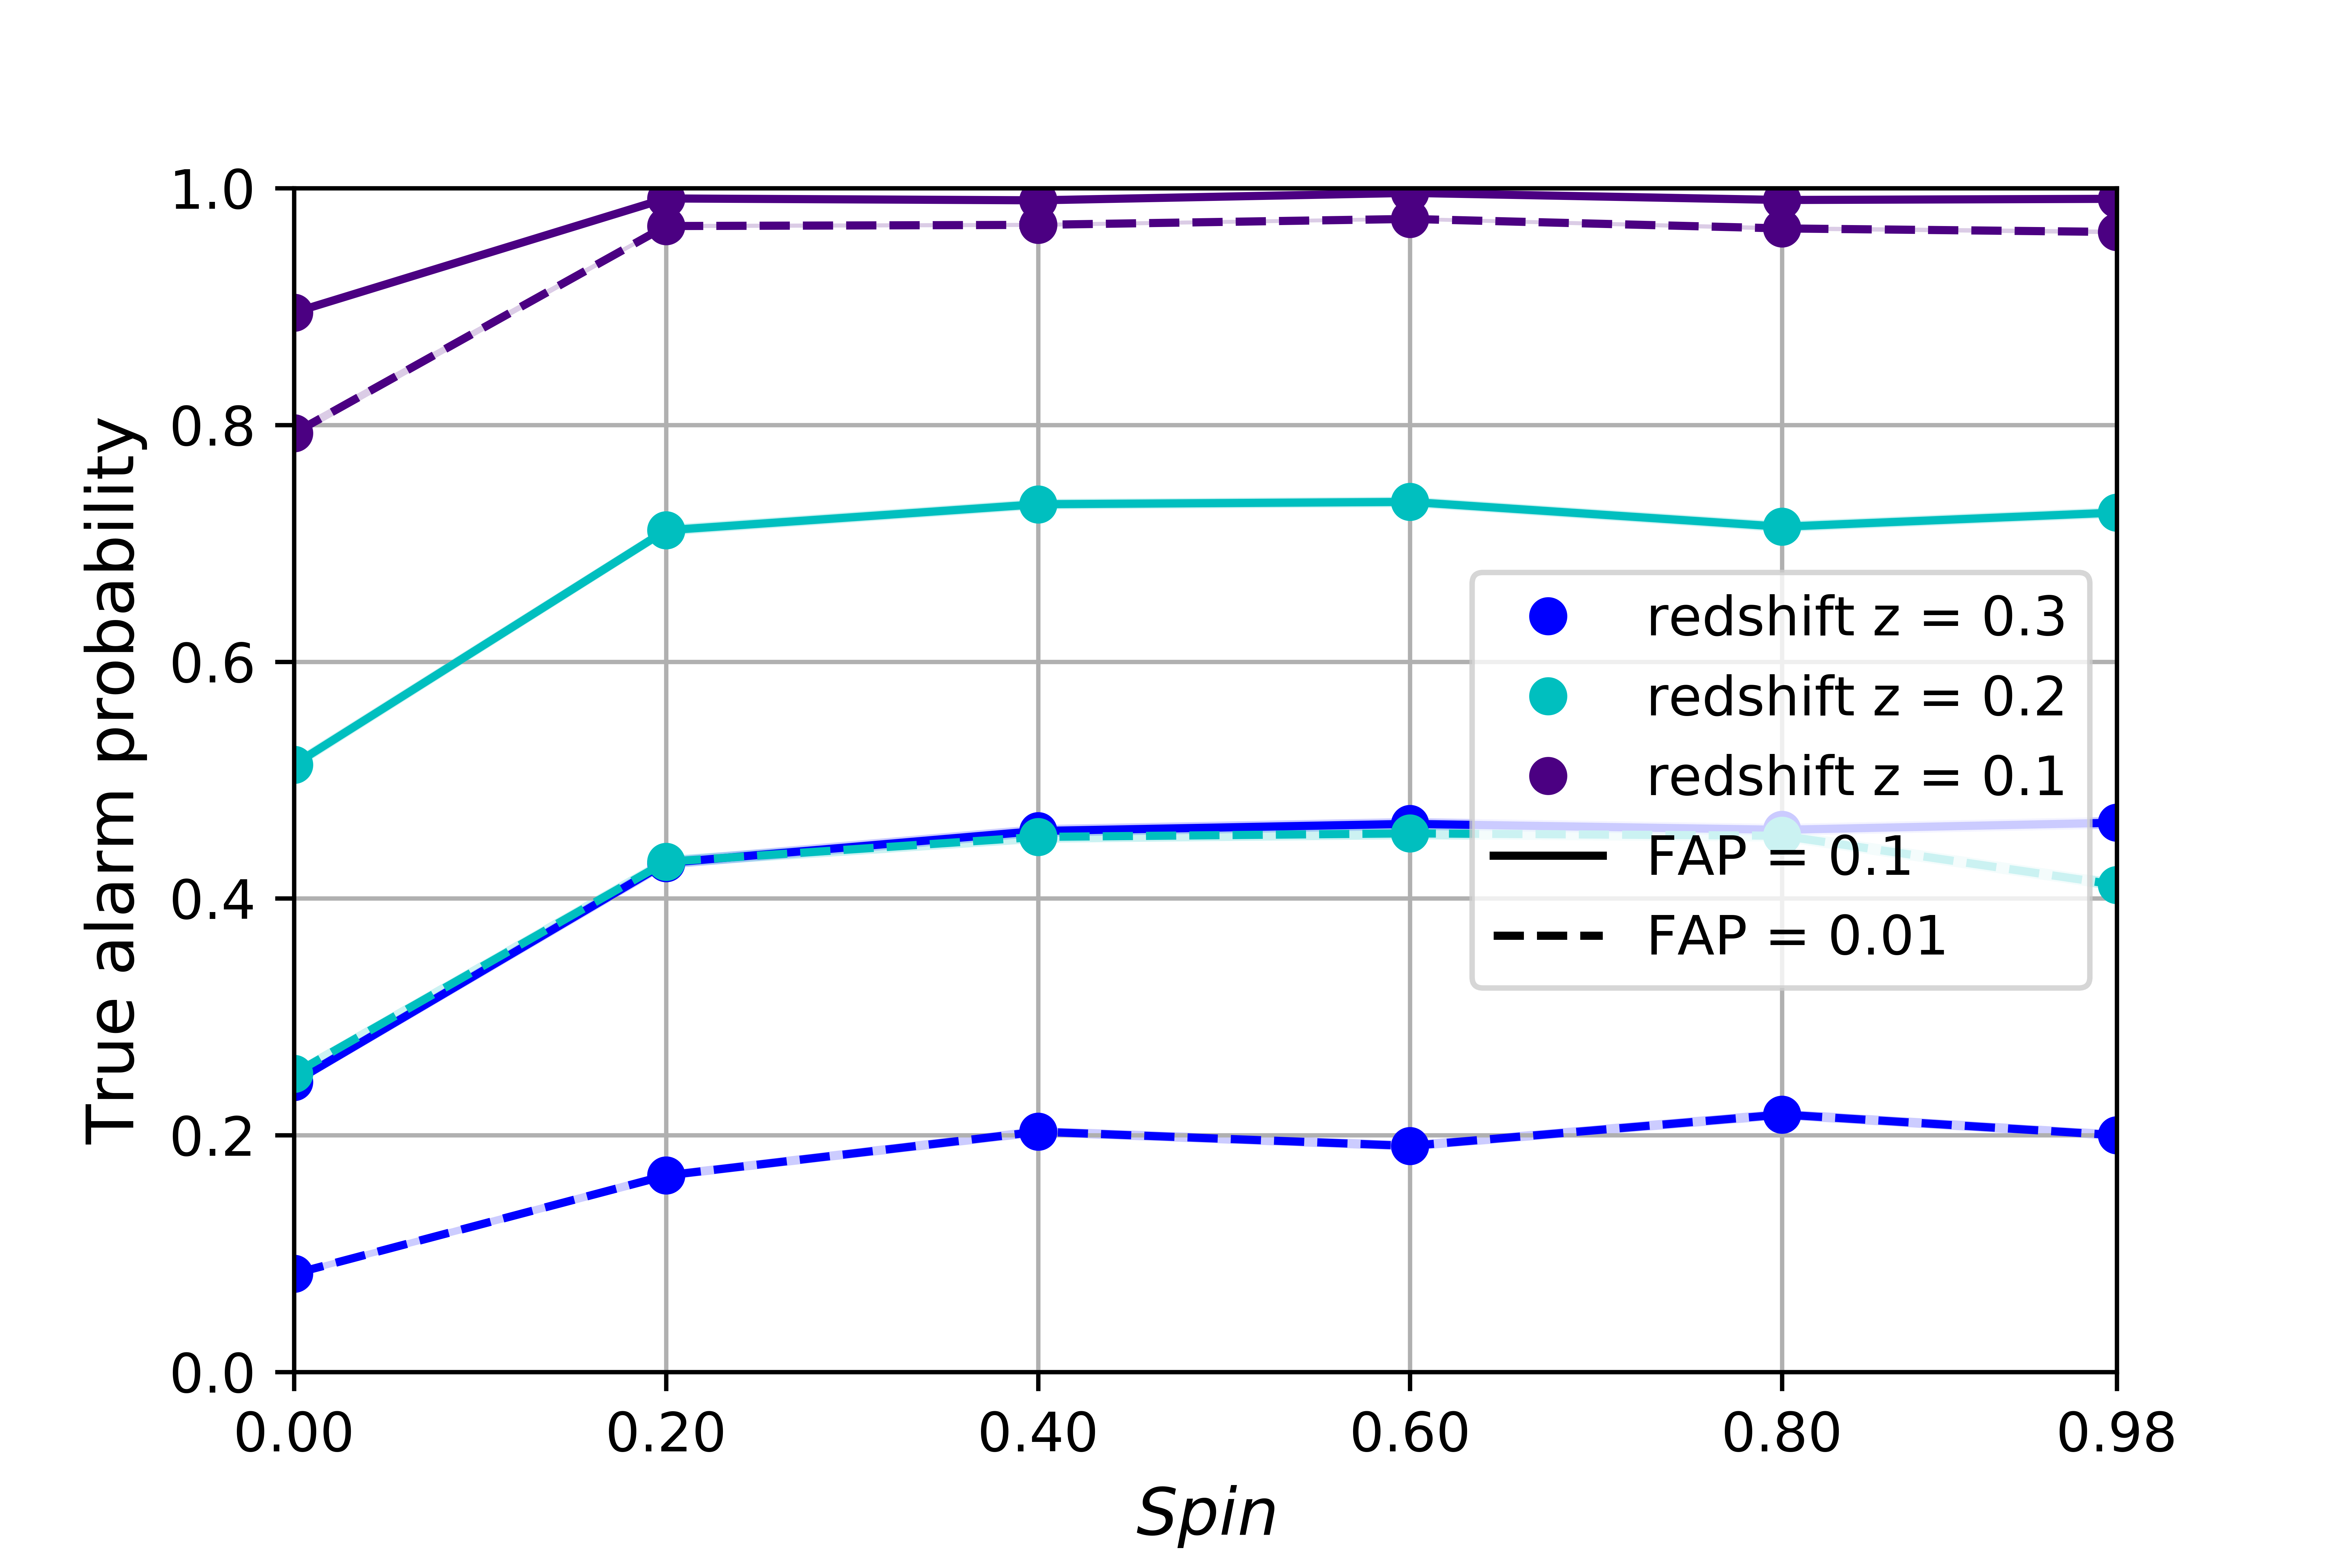
\includegraphics[width=.8\linewidth]{efficiency-Spin.png}
    \caption{\label{fig:EC-Spin}有效性曲线:含有固定大质量黑洞自旋不同模拟信号的测试数据集}
\end{figure}

\begin{figure}[!htbp]
\centering
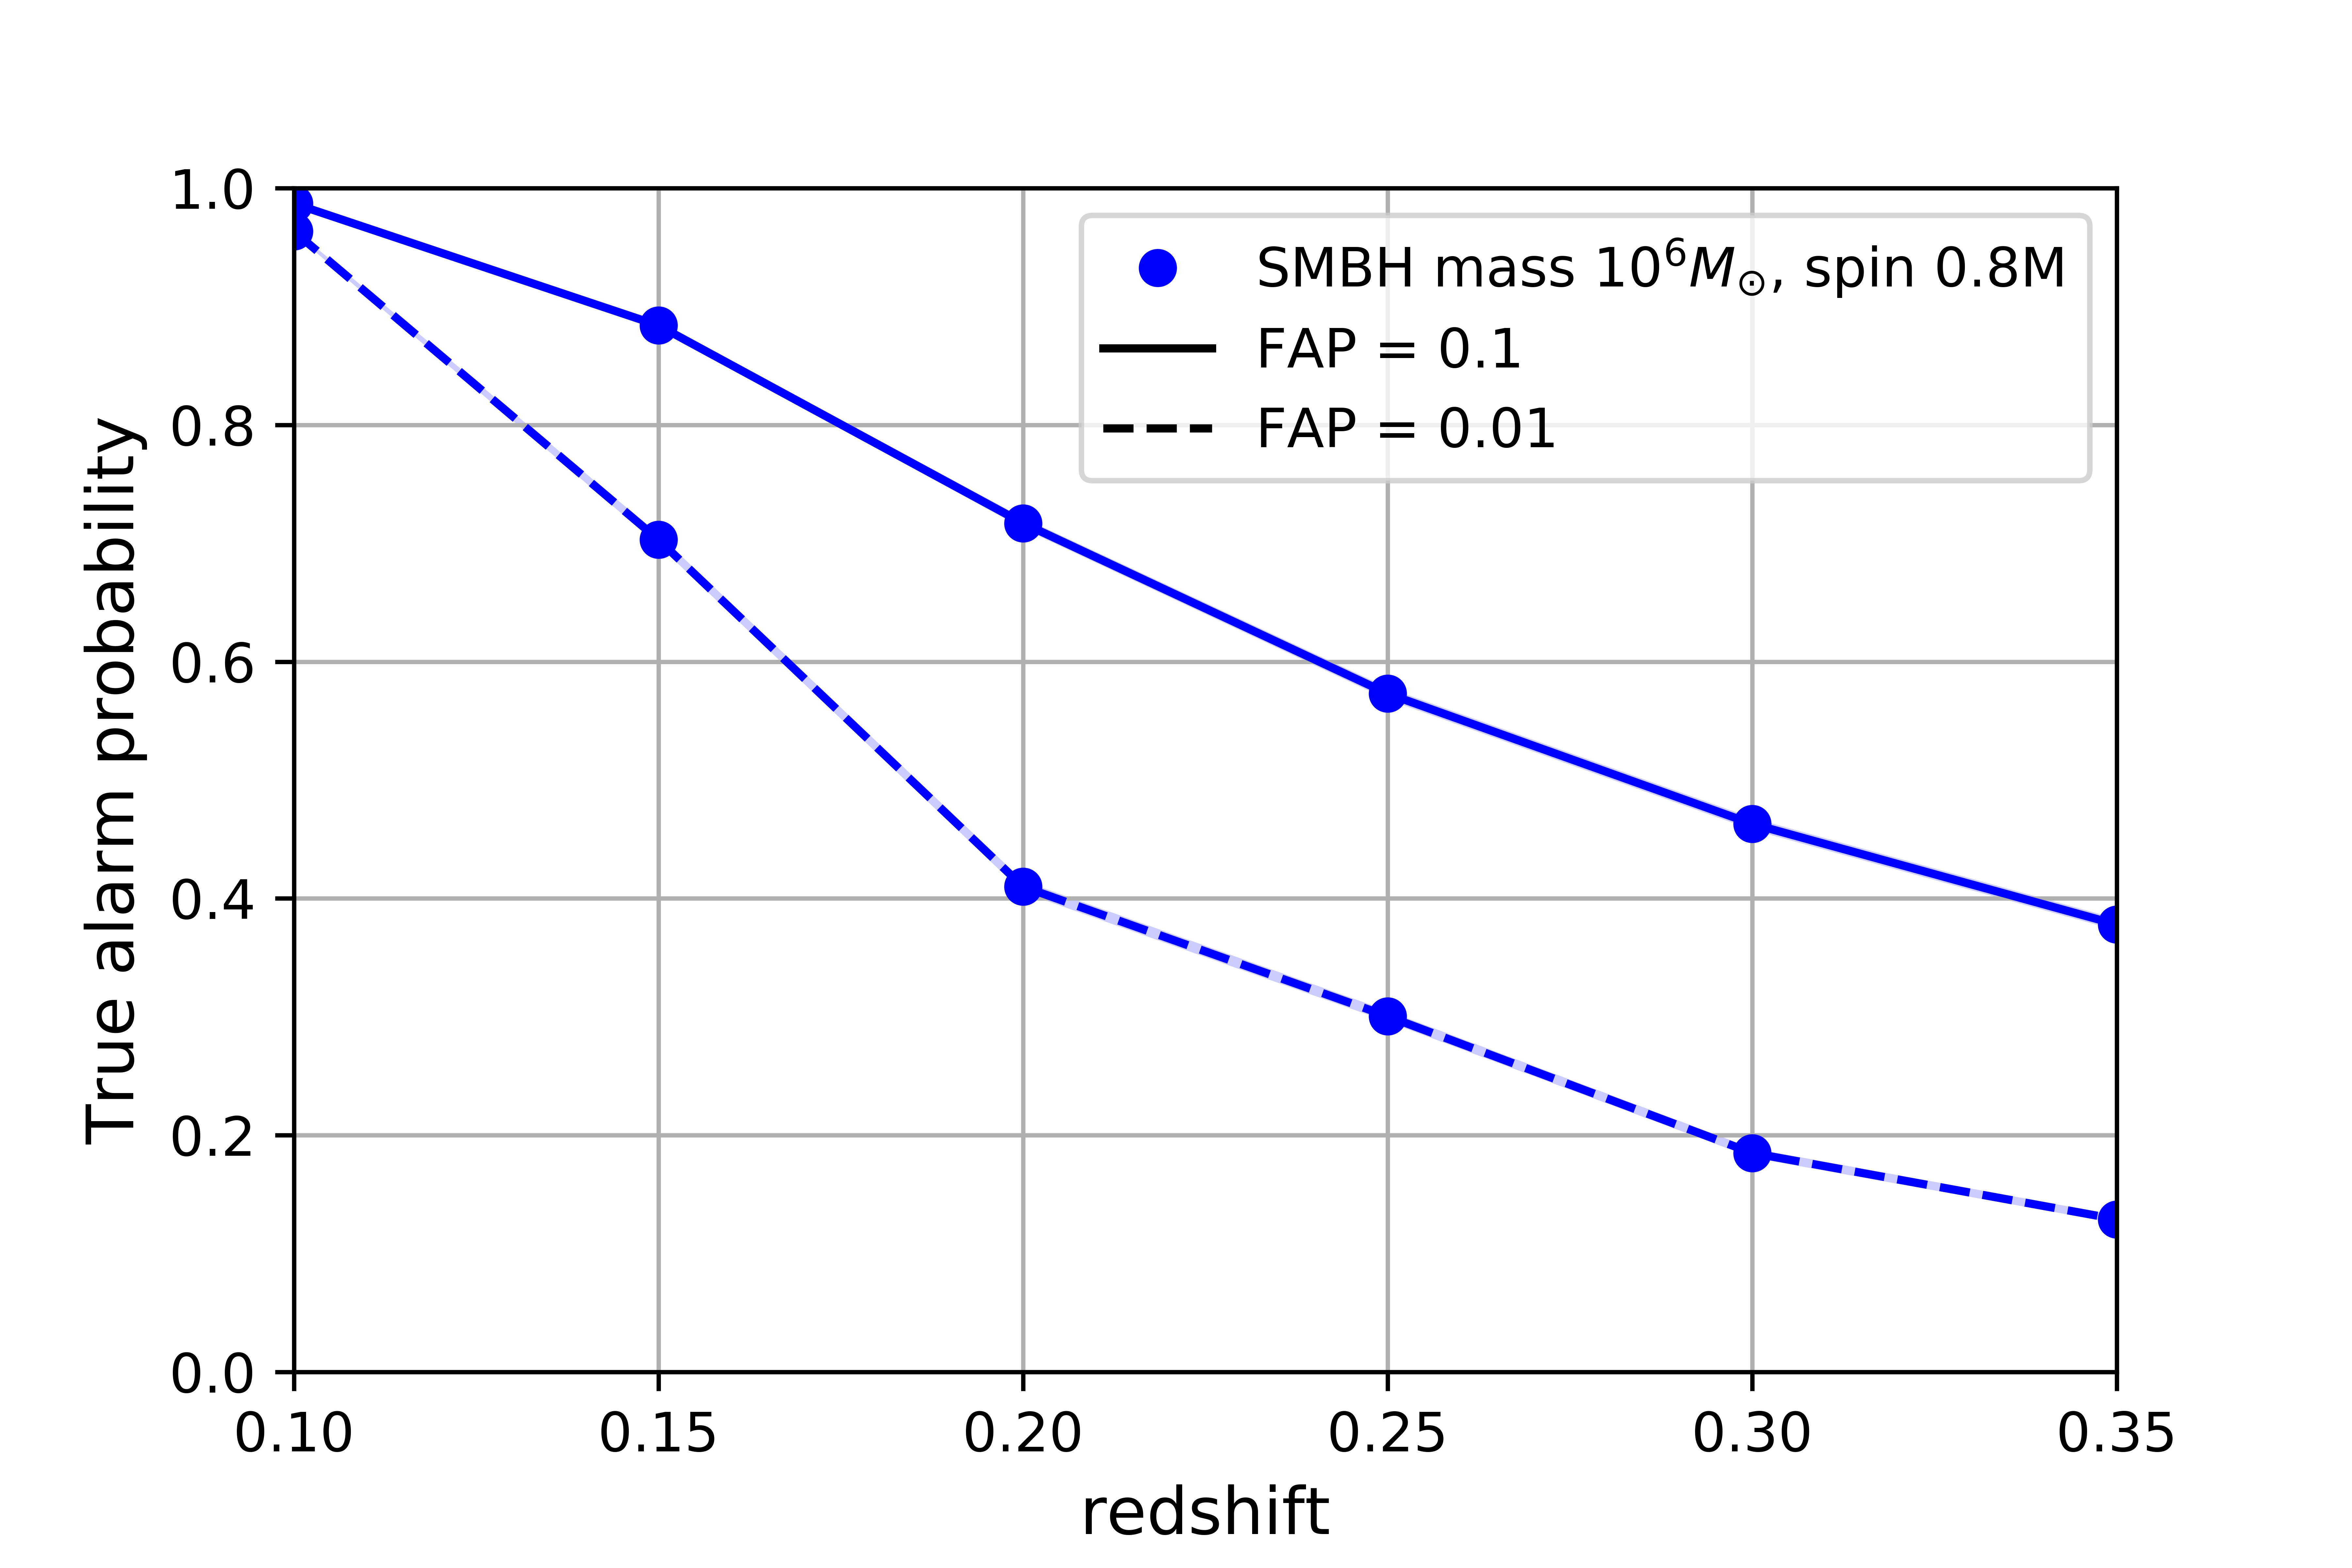
\includegraphics[width=.8\linewidth]{efficiency-Redshift.png}
\caption{\label{fig:EC-SNR}有效性曲线:含有固定信噪比不同模拟信号的测试数据集}
\end{figure}


%\chapter{EMRI信号参数估计}
%现有参数估计的方法及结果

%\chapter{数据处理流水线设计:以EMRI波源数据处理提出需求}